\documentclass[12pt]{report}
\usepackage[utf8]{inputenc}
\usepackage[margin=1.2in]{geometry}
\usepackage{graphicx}
\usepackage{float}
\usepackage{subcaption}
\usepackage{amsmath}
\usepackage{amssymb}
\usepackage{ulem}
\usepackage{bm}
\usepackage{framed}
\usepackage{xcolor}
\usepackage{ragged2e}
\usepackage{color}
\usepackage{soul}
\usepackage{cancel}
\graphicspath{ {images/} }
\setlength{\parskip}{1em}
\allowdisplaybreaks


\usepackage{titling}
\newcommand{\subtitle}[1]{%
	\posttitle{%
		\par\end{center}
	\begin{center}\large#1\end{center}
	\vskip0.5em}%
}

\newenvironment{blueframed}[1][blue]
{\def\FrameCommand{\fboxsep=\FrameSep\fcolorbox{#1}{white}}%
\MakeFramed {\advance\hsize-\width \FrameRestore}}
{\endMakeFramed}

\newenvironment{spmatrix}[1]
{\def\mysubscript{#1}\mathop\bgroup\begin{bmatrix}}
{\end{bmatrix}\egroup_{\textstyle\mathstrut\mysubscript}}

\title{Tutorial 6}
\subtitle
{
\textbf{keywords}: hypothesis testing, t-test, F-test, test statistic, critical value, confidence intervals, R-squared, interpretation of coefficients, multiple linear regression, reparameterisation

\textbf{estimated reading time}: 33 minutes
}
\author{Quang Bui}
\date{August 28, 2018}

\begin{document}

\maketitle

\section*{Question 1}
\noindent \textcolor{red}{\textit{Hypothesis test on a single parameter, the meanings of the size of a test and a confidence interval:}}

\noindent \textcolor{red}{Consider the classical linear regression model $$y_i = \beta_0 + \beta_1 x_i + u_i \quad i=1,2,\dots,n$$ A random sample of size $n=22$ is drawn and the estimated model based on this sample is:
\begin{align*}
	\hat{y}_i &= \underset{(3.1)}{5.4} + \underset{(1.5)}{3.2}x_i \quad i=1,2,\dots,22 \\
	R^2 &= 0.26 
\end{align*} (a) Test $H_0: \beta_1 = 0$ vs $H_1: \beta_1 \neq 0$ at the 5\%.}

\noindent For the simple linear regression model of $y$, $$y_i = \beta_0 + \beta_1 x_i + u_i \quad i=1,2,\dots,22$$ $\beta_1$ measures the true impact that $x$ has on $y$ (not holding any variable(s) constant because there are no other independent variables other than $x$ in this model). 

\noindent If $x$ does not truly impact $y$ then, $$\beta_1 = 0$$ but if it does,  $$\beta_1 \neq 0$$ After we estimate our model, $$\hat{y}_i = \underset{(3.1)}{5.4} + \underset{(1.5)}{3.2}x_i \quad i=1,2,\dots,22$$ we can perform this hypothesis test.

\noindent \textbf{State the null and alternative hypothesis}
\begin{align*}
H_0&: \beta_1 = 0 \\
H_1&: \beta_1 \neq 0
\end{align*}
\noindent \textbf{The test statistic and its distribution under $H_0$}
\begin{align*}
t &= \dfrac{\hat{\beta}_1 - \beta_1}{se(\hat{\beta}_1)} = \dfrac{\hat{\beta}_1 - 0}{se(\hat{\beta}_1)} = \dfrac{\hat{\beta}_1}{se(\hat{\beta}_1)} \sim t_{n-k-1} \quad under\ H_0 \\
n &= sample\ size = 22 \\
k &= number\ of\ regressors\ in\ the\ model = 1 \\
d.o.f &= n-k-1=20
\end{align*}
\noindent \textbf{Calculate the test statistic}
$$t_{calc} = \dfrac{\hat{\beta}_1}{se(\hat{\beta}_1)} = \dfrac{3.2}{1.5} = 2.1333$$
\noindent \textbf{Critical value and rejection region}

\noindent $5\%\ significance\ level\ \therefore \alpha = 0.05$, two-sided t-test

\noindent Since we are performing a t-test, the critical value(s) (which bounds the rejection region) come from a t-distribution. The t-distribution of interest in this hypothesis test, is one with $degrees\ of\ freedom\ = n - k - 1 = 22 - 2 = 20$. 


\begin{figure}[H]
	\centering
	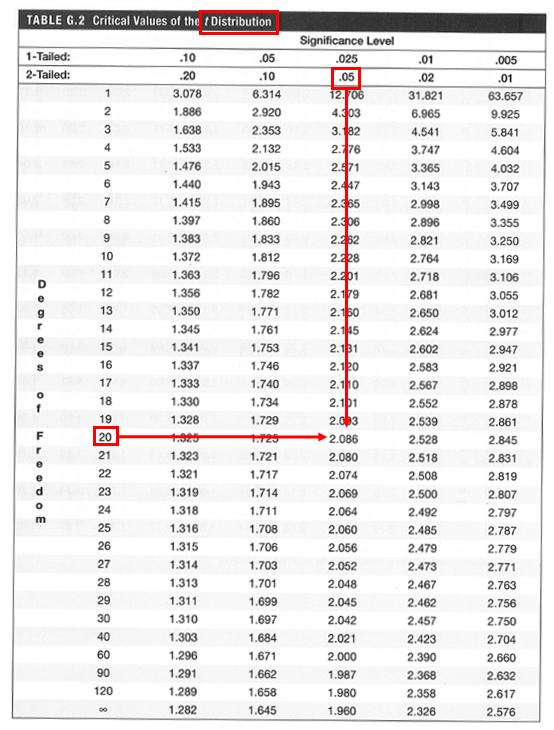
\includegraphics{tute6_q1_4}
\end{figure}
\vspace{-\baselineskip} \noindent (Note: If the degrees of freedom cannot be found in the statistics table, we take a conservative approach and choose the closest available degrees of freedom less than what we need.)
\noindent From the statistics table: \begin{align*}
	+t_{crit} &= t_{20,0.975} = 2.086 \\
	-t_{crit} &= t_{20,0.025} = -2.086
\end{align*}
\noindent To obtain the critical value using EViews,
$$Command\ window:\ =@qtdist(0.975,20)$$
\begin{figure}[H]
	\centering
	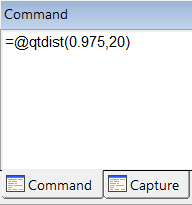
\includegraphics{tute6_q1_5}
\end{figure}
\vspace{-\baselineskip}\centering $(press\ Enter\ to\ execute)$
\justify and the value appears in the bottom left corner,
\begin{figure}[H]
	\centering
	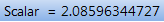
\includegraphics{tute6_q1_6}
\end{figure}
\vspace{-\baselineskip}
\noindent From EViews: \begin{align*}
+t_{crit} &= t_{20,0.975} = 2.086 \\
-t_{crit} &= t_{20,0.025} = -2.086
\end{align*}
\noindent For a two-sided t-test, we reject $H_0$ if,
$$t_{calc} > +t_{crit}$$
$$or$$
$$t_{calc} < -t_{crit}$$
\noindent \textbf{Conclusion}

\noindent Since $t_{calc} = 2.1333 > +t_{crit} = 2.086$, we reject the null at the 5\% significance level and conclude that there is sufficient evidence from our sample to suggest that $x$ has a statistically significant impact on $y$.

\newpage
\noindent \textcolor{red}{(b) Construct a 95\% confidence interval for $\beta_1$}
$$\hat{\beta}_1 \pm t_{crit} \times se(\hat{\beta}_1)$$
$$\hat{\beta}_1 \pm t_{n-k-1,1-\frac{\alpha}{2}} \times se(\hat{\beta}_1)$$
$$\hat{\beta}_1 \pm t_{20,0.975} \times se(\hat{\beta}_1)$$
$$3.2 \pm 2.086 \times 1.5$$
$$[0.071,6.329]$$

\noindent \textcolor{red}{(c) Suppose that you learn that $y$ and $x$ are independent. Would you be surprised? Explain.}

\noindent If $y$ and $x$ are independent then $x$ should not effect $y$ i.e. $\beta_1 = 0$, but we rejected $$H_0: \beta_1 = 0$$ and concluded that $x$ has a statistically significant impact on $y$ at the 5\% significance level. Setting our significance level at 5\% $$\alpha=0.05$$ means that there is only a 5\% chance of rejecting the null when it is true $\therefore$ we would be surprised.

\noindent Concretely, we have evidence from this sample to reject the null hypothesis that $x$ has no impact on $y$ at the 5\% significance level. We could have wrongly rejected $H_0$ when it is true (Type I error), but since we performed this test at the 5\% significance level, this error occurs with only a 5\% probability, $$P(Type\ I\ error) = \alpha = 0.05$$ Given that $y$ and $x$ are independent $\therefore$ $x$ has no true impact on $y$ i.e. $\beta_1 = 0$, if we applied repeated sampling and performed the same hypothesis test across many more samples, we would find that $H_0$ is wrongly rejected in 5\% of these samples.

\noindent \textcolor{red}{(d) Suppose that you learn that $y$ and $x$ are independent and many samples of $n=22$ are drawn, regressions estimated, and (a) and (b) answered. In what fraction of the samples would $H_0$ from (a) be rejected? In what fraction of samples would the value $\beta_1 = 0$ be included in the confidence interval from (b)?}

\noindent The significance level, $\alpha$, is the probability of rejecting the null hypothesis when it is true. Since we set $\alpha = 0.05$, this means there is a 5\% chance that we reject $H_0: \beta_1=0$ when it is true.Therefore, we would reject $H_0: \beta_1=0$ in 5\% of the samples.

\noindent The true value of $\beta_1$ will lie in 95\% of the confidence intervals. If we learn that $y$ and $x$ are independent, then the true value of $\beta_1$ is $0$, so $\beta_1 = 0$ would lie in 95\% of the confidence intervals.

\newpage
\section*{Question 2}
\noindent \textcolor{red}{\textit{Practice with t-test and F-test:} (This is based on problem 3 at the end of Chapter 3 of the textbook): The following multiple regression model was used to study the trade-off between time spent sleeping and working and to look at other factors affecting sleep: $$sleep = \beta_0 + \beta_1 totwrk + \beta_2 educ + \beta_3 age + u$$ where $sleep$ and $totwrk$ are measured in minutes per week and $educ$ and $age$ are measured in years.}

\noindent \textcolor{red}{(a) If adults trade-off sleep for work, what is the sign of $\beta_1$?}

\noindent Keeping education and age constant, if an adult who trades off sleep for work, we would expect $\beta_1$ to be negative.

\noindent \textcolor{red}{(b) What signs do you think $\beta_2$ and $\beta_3$ will have?}

\noindent $\beta_2$ measures the impact of education on time spent sleeping after controlling for years of education and age. So, if we take 2 individuals of the same age and who both work the same number of hours each week, would we expect the more educated individual to sleep more or less? If we consider that less educated people perhaps work more physical hours and need more sleep to recover, then we could say that $\beta_2$ has a negative sign.

\noindent $\beta_3$ measures the impact of age on time spent sleeping after controlling for hours spending working each week and years of education. So, if we take 2 individuals with the same years of education and who both work the same number of hours each week, would we expect the older individual to sleep more or less? This is hard to say. All else equal, older people generally need more sleep, but we also know that university students sleep more than 25-35 year olds.

\noindent \textcolor{red}{(c) Using data from a random sample of 706 adults, we have estimated the following equation: \begin{align}
	\widehat{sleep} &= \underset{(112.27)}{3638.25} - \underset{(0.017)}{0.148}totwrk - \underset{(5.88)}{11.13}educ + \underset{(1.45)}{2.20}age \\
	R^2 &= 0.113 \quad SSR = 123455057 \nonumber
	\end{align} Test the hypothesis that adults do not trade-off sleep for work against the alternative that they do at the 1\% level of significance.
}

\noindent If adults do not trade-off sleep for work then, $$\beta_1 = 0$$ We test this against the alternative hypothesis that they do trade sleep for work, $$\beta_1 < 0$$ Here we are performed a 1-sided t-test at the 1\% level of significance.

\noindent \textbf{State the null and alternative hypothesis}
\begin{align*}
H_0&: \beta_1 = 0 \\
H_1&: \beta_1 < 0
\end{align*}
\noindent \textbf{The test statistic and its distribution under $H_0$}
\begin{align*}
t &= \dfrac{\hat{\beta}_1 - \beta_1}{se(\hat{\beta}_1)} = \dfrac{\hat{\beta}_1 - 0}{se(\hat{\beta}_1)} = \dfrac{\hat{\beta}_1}{se(\hat{\beta}_1)} \sim t_{n-k-1} \quad under\ H_0 \\
n &= sample\ size = 706 \\
k &= number\ of\ regressors\ in\ the\ model = 3 \\
d.o.f &= n-k-1=706 - 3 - 1 = 702
\end{align*}
\noindent \textbf{Calculate the test statistic}
$$t_{calc} = \dfrac{\hat{\beta}_1}{se(\hat{\beta}_1)} = -\dfrac{0.148}{0.017} = -8.706$$
\noindent \textbf{Critical value and rejection region}

\noindent $1\%\ significance\ level\ \therefore \alpha = 0.01$, one-sided t-test (one the left side because $H_1: \beta_1 < 0$)

\noindent Since we are performing a t-test, the critical value(s) (which bounds the rejection region) come from a t-distribution. The t-distribution of interest in this hypothesis test, is one with $degrees\ of\ freedom\ = n - k - 1 = 706 - 3 - 1 = 702$. Since $d.o.f = 702$ is not in the statistics table, we take a conservative approach and choose the closest available degrees of freedom less than 702 i.e. $d.o.f=120$. 


\begin{figure}[H]
	\centering
	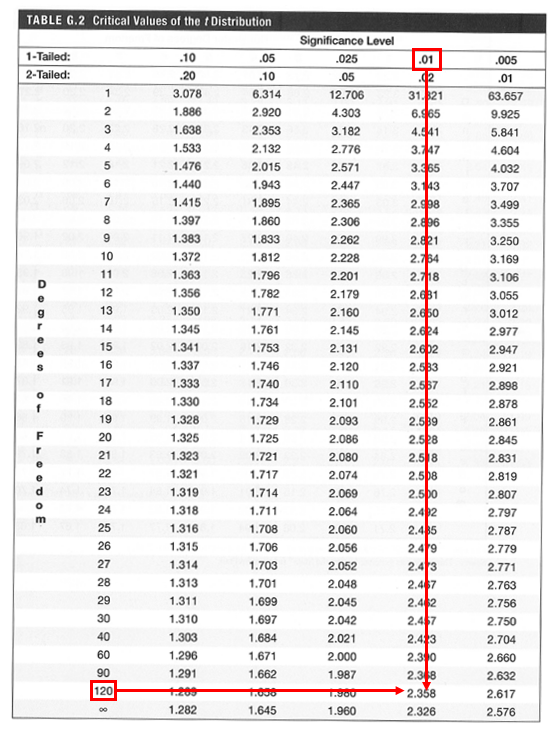
\includegraphics{tute6_q2_4}
\end{figure}
\vspace{-\baselineskip}
\noindent From the statistics table: \begin{align*}
-t_{crit} &= -2.358 
\end{align*} (We are only concerned with the negative critical value because we are performing a one-sided t-test on the left side.)

\noindent To obtain the critical value using EViews,
$$Command\ window:\ =@qtdist(0.01,702)$$
\begin{figure}[H]
	\centering
	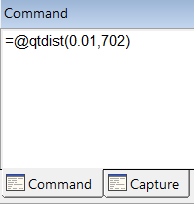
\includegraphics{tute6_q2_5}
\end{figure}
\vspace{-\baselineskip}\centering $(press\ Enter\ to\ execute)$
\justify and the value appears in the bottom left corner,
\begin{figure}[H]
	\centering
	
\includegraphics{tute6_q2_6}
\end{figure}
\vspace{-\baselineskip}
\noindent From EViews: \begin{align*}
+t_{crit} &= t_{702,0.01} = -2.3317
\end{align*}
\noindent For a one-sided t-test on the negative side, we reject $H_0$ if,
$$t_{calc} < -t_{crit}$$
\noindent \textbf{Conclusion}

\noindent Since $t_{calc} = -8.706 > -t_{crit} = -2.3317$, we reject the null at the 1\% significance level and conclude that there is sufficient evidence from our sample to suggest that there is a trade-off between work time and sleep.

\noindent \textcolor{red}{(d) Construct a 95\% confidence interval for $\beta_3$. Interpret the confidence interval.}
$$\hat{\beta}_3 \pm t_{crit} \times se(\hat{\beta}_3)$$
$$\hat{\beta}_3 \pm t_{n-k-1,1-\frac{\alpha}{2}} \times se(\hat{\beta}_3)$$
$$\hat{\beta}_3 \pm t_{702,0.975} \times se(\hat{\beta}_3)$$
$$2.20 \pm 1.980 \times 1.45$$
$$[-0.671,5.071]$$
\noindent In repeated samples, 95\% of the sample will contain $\beta_3$. The range from our confidence interval is an \textit{interval estimate} of $\beta_3$. Since the interval estimate includes $0$, this means that $age$ is not a statistically significant predictor of sleep time after controlling for work and education. ($\hat{\beta}_3$ is not statistically significantly different from 0 at the 5\% significance level.)

\noindent \textcolor{red}{(e) We have also estimated the following regression: \begin{align}
	\widehat{sleep} &= \underset{(38.91)}{3586.38} - \underset{(0.017)}{0.151}totwrk \\
	SSR &= 124858119 \nonumber
	\end{align} Test the joint hypothesis given work time, education \& age have no effect on sleep time versus the alternative that at least one of them does (when the others are constant). Perform this test at the 5\% level of significance.}

\noindent \noindent If, after controlling for $work$, $educ$ \& $age$ jointly have no effect on sleep time then,
$$sleep = \beta_0 + \beta_1 totwrk + \xcancel{\beta_2 educ} + \xcancel{\beta_3 age} + u$$
$$\beta_2 = 0, \beta_3 = 0$$ 
\noindent but if at least one of $educ$ and $age$ does effect sleep then,
$$\beta_2 \neq 0\ and/or\ \beta_3 \neq 0$$ Unlike the t-test, which testings a single linear restriction, the F-test is used when we wish to perform a hypothesis test of multiple linear restrictions. Since we have 2 linear restrictions to test, we use the F-test.

\noindent The null and alternative hypothesis are stated as, \begin{align*}
	H_0&: \beta_2 = \beta_3 = 0 \\
	H_1&: at\ least\ one\ of\ \beta_2\ or\ \beta_3\ does\ not\ equal\ 0
\end{align*} The model when $H_0$ is true i.e without $educ$ and $age$, $$sleep = \beta_0 + \beta_1 totwrk + u$$ is called the \textit{restricted model} because it imposes the 2 linear restrictions that $\beta_2 = \beta_3 = 0$, while the model without any restrictions imposed, $$sleep = \beta_0 + \beta_1 totwrk + \beta_2 educ + \beta_3 age + u$$ is called the \textit{unrestricted model}.

\newpage
\noindent \textbf{Unrestricted model (the model before imposing restrictions)}:
$$sleep = \beta_0 + \beta_1 totwrk + \beta_2 educ + \beta_3 age + u$$ \textbf{Restricted model (the model after imposing restrictions)}: $$sleep = \beta_0 + \beta_1 totwrk + u$$ \textbf{State the null and alternative hypothesis}
\begin{align*}
H_0&: \beta_2 = \beta_3 = 0 \\
H_1&: at\ least\ one\ of\ \beta_2\ or\ \beta_3\ does\ not\ equal\ 0
\end{align*} \textbf{The test statistic and its distribution under $H_0$}
$$F = \dfrac{(SSR_r - SSR_{ur})/q}{SSR_{ur}/(n-k-1)} = \dfrac{(SSR_r - SSR_{ur})/2}{SSR_{ur}/(706-3-1)} \sim F_{q,n-k-1} \quad under\ H_0$$
\begin{align*}
n &= sample\ size = 706 \\
k &= number\ of\ regressors\ in\ the\ unrestricted\ model = 3 \\
q &= number\ of\ restrictions\ = 2 \\
SSR_{r} &= sum\ of\ squared\ residuals\ from\ estimated\ restricted\ model \\
SSR_{ur} &= sum\ of\ squared\ residuals\ from\ estimated\ unrestricted\ model
\end{align*} \textbf{Calculate the test statistic}
\begin{align*}
	SSR_r &= 124858119 \\
	SSR_{ur} &= 123455057
\end{align*}
$$F_{calc} = \dfrac{(SSR_r - SSR_{ur})/2}{SSR_{ur}/(706-3-1)} = \dfrac{(124858119 - 123455057)/2}{123455057/(702)} = 3.989$$ \textbf{Critical value and rejection region}

\noindent $5\%\ significance\ level\ \to \alpha = 0.05$

\noindent To obtain the critical value using the Stats Table, locate the F distribution table at the 5\% significance level,
$$Numerator\ d.o.f = 2$$
$$Denominator\ d.o.f = 702$$
\noindent Since 702 is not in the table, we take a conservative approach and choose the closest available degrees of freedom less than 702 i.e. $d.o.f=120$. 
\begin{figure}[H]
	\centerline{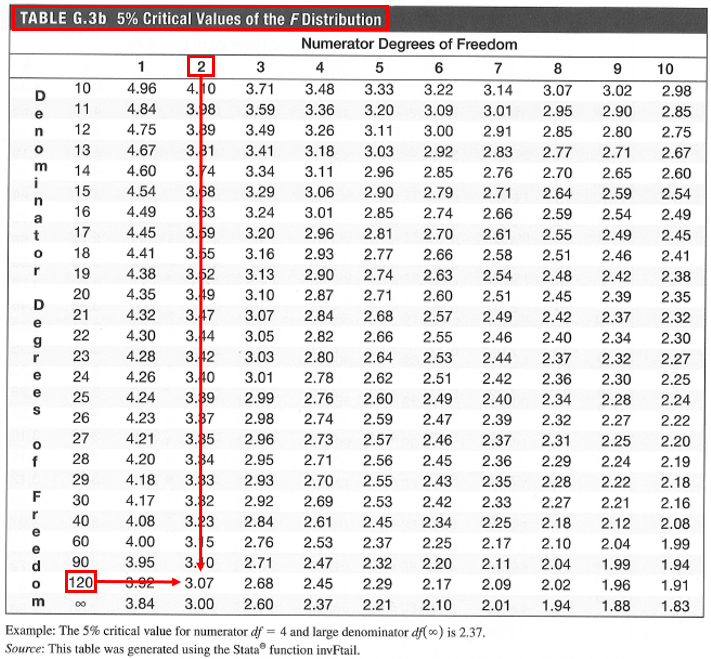
\includegraphics{tute6_q2_7}}
\end{figure}
\vspace{-\baselineskip}
\noindent To obtain the critical value using EViews,
$$Command\ window:=@qfdist(0.95,2,702)$$
\begin{figure}[H]
	\centerline{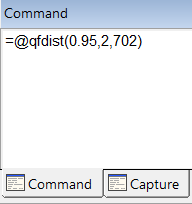
\includegraphics{tute6_q2_8}}
\end{figure}
\vspace{-\baselineskip} $$Press\ Enter\ to\ execute\ and\ the\ cv\ appears\ at\ the\ bottom\ left\ corner$$ \begin{figure}[H]
	\centerline{
\includegraphics{tute6_q2_9}}
\end{figure}
\vspace{-\baselineskip}
$$F_{crit}\ (from\ Stat\ Table) = 3.07$$
$$F_{crit}\ (from\ EViews) = 3.0086$$ \noindent Rejection rule: 

\noindent Comparing the calculated test statistic with the critical value, we reject $H_0$ if,
$$F_{calc} > F_{crit}$$
\noindent \textbf{Conclusion}

\noindent Since $F_{calc}=3.989 > F_{crit}=3.07$, we reject the null at the 5\% significance level and conclude that given work time, at least one of education or age has a significant effect on sleep time.

\noindent \textcolor{red}{(f) Compute the $R^2$ of regression (2).} $$(Discuss\ in\ class)$$

\noindent \textcolor{red}{(g) Suppose that someone suggests that one year of education keeping all else constant has the same effect but with opposite sign of the effect of one more year of age keeping all else constant. That is, $\beta_2 = -\beta_3$. Explain how you would test this hypothesis with an F-test. You need to state the alternative hypothesis that can be tested with an F-test, specify any extra regression that you need to estimate, and explain how you would use the results of that regression to test this hypothesis.} $$(Discuss\ in\ class)$$

\noindent \textcolor{red}{(h) Suppose the alternative hypothesis of interest was $\beta_2 < -\beta_3$. Explain how you would test $H_0: \beta_2 = -\beta_3$ against this one-sided alternative.}

\noindent The null hypothesis is,
$$H_0: \beta_2 + \beta_3 = 0$$ 
and although it involves two parameters, it tests only one restriction. The alternative is, 
$$H_1: \beta_2 + \beta_3 < 0$$ so we cannot use the F test because the F test provides inference against $\beta_2 + \beta_3 \neq 0$. In such cases that we have only one restriction about a linear combination, we use a reparameterisation trick: 
$$Define\ \delta = \beta_2 + \beta_3 \implies \beta_2 = \delta - \beta_3$$
Subsitute for $\beta_2$ in the population model and re-arrange, \begin{align*}
	sleep &= \beta_0 + \beta_1 totwrk + \beta_2 educ + \beta_3 age + u \\
	&= \beta_0 + \beta_1 totwrk + (\delta - \beta_3) educ + \beta_3 age + u \\
	&= \beta_0 + \beta_1 totwrk + \delta educ - \beta_3 educ + \beta_3 age + u \\
	&= \beta_0 + \beta_1 totwrk + \delta educ + \beta_3 (age - educ) + u 
\end{align*} you will see that $\delta$ becomes the coefficient of one of the explanatory variables in the reparameterised model. \begin{figure}[H]
	\centerline{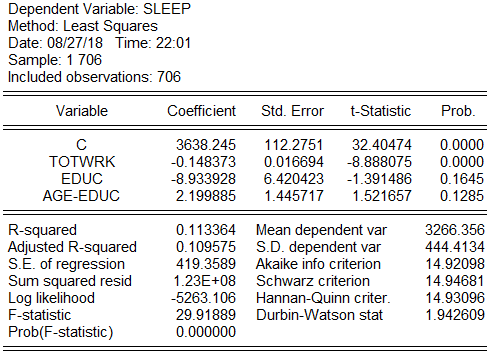
\includegraphics{tute6_q2_10}}
\end{figure}
\vspace{-\baselineskip} $$\widehat{sleep} = \hat{\beta}_0 + \hat{\beta}_1 totwrk + \hat{\delta} educ + \hat{\beta}_3 (age - educ)$$ where $$\hat{\delta} = -8.9339 \quad se(\hat{\delta}) = 6.4204$$
\noindent You can see that testing $\delta = 0$ against $\delta < 0$ can be performed with a simple t test in this reparameterised model,
\begin{align*}
	H_0&: \delta = 0 \quad (same\ as\ \beta_2 + \beta_3 = 0) \\
	H_1&: \delta < 0 \quad (same\ as\ \beta_2 + \beta_3 < 0
\end{align*}
$$(one-sided\ t\ test)$$
\noindent \textbf{The test statistic and its distribution under $H_0$}
$$t = \dfrac{\hat{\delta} - \delta}{se(\hat{\delta})} = \dfrac{\hat{\delta}}{se(\hat{\delta})} \sim t_{n-k-1} \quad under\ H_0$$
\begin{align*}
n &= sample\ size = 706 \\
k &= number\ of\ regressors\ in\ the\ model = 3
\end{align*}

\noindent \textbf{Calculate the test statistic}
$$t_{calc} = -\dfrac{8.9339}{6.4204} = -1.3915$$
\noindent \textbf{Critical value and rejection region}

\noindent $5\%\ significance\ level\ \to \alpha = 0.05$ $$degrees\ of\ freedom = n - k - 1 = 702$$
\noindent Since 702 is not in the table, we take a conservative approach and choose the closest available degrees of freedom less than 702 i.e. $d.o.f=120$. 

\noindent \textit{Note: This gives us $+t_{crit}$ but we\ need\ $-t_{crit}$\ since\ we\ are\ performing\ a\ one\ side\ test\ on\ the\ negative\ side.}

\noindent From Stat Table:
$$-t_{crit} = -1.658$$
\noindent Rejection rule: 

\noindent Comparing the calculated test statistic with the critical value, we reject $H_0$ if,
$$t_{calc} < -t_{crit}$$
\noindent Comparing the p-value with the significance level, we reject $H_0$ if,
$$\dfrac{p-value}{2} < \alpha = 0.05$$ $$(divide\ p\ value\ by\ 2\ for\ one\ sided\ t\ test)$$
\noindent \textbf{Conclusion}

\noindent Since $t_{calc} =-1.3915 > -t_{crit} = -1.658$, we do not reject the null at the 5\% significance level and conclude that there is insufficient evidence from our sample to suggest that $\beta_2 + \beta_3 < 0$.







\end{document}
